% This is samplepaper.tex, a sample chapter demonstrating the
% LLNCS macro package for Springer Computer Science proceedings;
% Version 2.21 of 2022/01/12
%
\documentclass[runningheads]{llncs}
%
\usepackage[T1]{fontenc}
% T1 fonts will be used to generate the final print and online PDFs,
% so please use T1 fonts in your manuscript whenever possible.
% Other font encondings may result in incorrect characters.
%
\usepackage{graphicx}
\usepackage{bm}
% Used for displaying a sample figure. If possible, figure files should
% be included in EPS format.
%
% If you use the hyperref package, please uncomment the following two lines
% to display URLs in blue roman font according to Springer's eBook style:
%\usepackage{color}
%\renewcommand\UrlFont{\color{blue}\rmfamily}
%
\usepackage{subcaption}
\usepackage{multirow}
\usepackage{cite}
\usepackage{breqn}
\usepackage{amsmath,amssymb,amsfonts}
\usepackage{textcomp}
\usepackage{algorithmic}
\usepackage{soul}
\usepackage{float}
\usepackage{amsmath} % assumes amsmath package installed
\usepackage{amssymb} 
\usepackage{array}
%\usepackage{algpseudocode}
\usepackage{blindtext}
\usepackage{color}
\usepackage{algorithm}
\usepackage{epstopdf}
\restylefloat{algorithm}
\usepackage{hyperref}
\usepackage{subcaption}
\newcommand{\INDSTATE}[1][1]{\STATE\hspace{#1\algorithmicindent}}
\newcounter{mytempeqncnt}
\def\BibTeX{{\rm B\kern-.05em{\sc i\kern-.025em b}\kern-.08em
		T\kern-.1667em\lower.7ex\hbox{E}\kern-.125emX}}

%\DeclareUnicodeCharacter{034F}{}

\begin{document}



%
\title{A systematic approach to predicting acceptance of banking products using neural networks, ensemble models, and explainability techniques.}
%
\titlerunning{Systematic process for predicting acceptance of banking products}
% If the paper title is too long for the running head, you can set
% an abbreviated paper title here
%
%\author{Andrés Encalada\inst{1} \and
%Karen Ortiz\inst{2}}
%
%\authorrunning{F. Author et al.}
% First names are abbreviated in the running head.
% If there are more than two authors, 'et al.' is used.
%
%\institute{Universidad Politécnica Salesiana, Cuenca, Ecuador \\ 
%\email{bencaladaa@est.ups.edu.ec} ,
%\email{kortizp4@est.ups.edu.ec}}
%
\maketitle              % typeset the header of the contribution
%
\begin{abstract}
In the banking sector, identifying customers who will take out fixed-term deposits helps optimize marketing resources. Datasets are often high-dimensional and class-imbalanced, which can lead to biased models. To address these challenges, CRISP-ML(Q) is the proposed process. Phase 1 integrates data preparation techniques such as PCA for dimensionality reduction, clustering, and SMOTE for class balancing. In phase 2, a comparison is made between traditional learning algorithms (Random Forest and KNN), a neural network architecture, and a Stacking Generalization approach. In phase 3, performance is validated using metrics and XAI techniques with SHAP values to interpret the model's decisions.
The experiment uses the “Banking Marketing” dataset from the UCI machine learning repository, which contains real data from a Portuguese banking institution. 
Model performance is evaluated using precision, accuracy, recall, F1 score, and AUC-ROC.
The results reveal the effectiveness of the different methods. This work lays the foundation for the implementation of an explainable model for fintech organizations in a real-time environment and for the exploration of transformer-based architectures for tabular data to improve predictive sensitivity.

\keywords{Neural Network  \and Ensamble Learning \and PCA \and SMOTE \and CRISP-ML(Q) \and Bank Marketing.}
\end{abstract}
%
%
%
\section{Introduction}

In the age of digital banking, customer information is more valuable than products, and banks invest millions of dollars annually in direct marketing campaigns that often fail and generate customer fatigue. The main challenge lies in identifying which customers are likely to subscribe to a fixed-term deposit, a task complicated by the strong class imbalance between successful and unsuccessful cases, which biases traditional learning algorithms \cite{moro2014data}.\\

Addressing this problem improves operational efficiency, increases the return on investment (ROI) of telemarketing campaigns, and enhances customer experience by reducing unnecessary interactions. This work proposes an intelligent adaptive system based on the methodology of \cite{hurtado2024intelligent}, extended through a comparative analysis of traditional models, ensemble methods, and artificial neural networks. Our approach integrates a preprocessing pipeline that combines dimensionality reduction, clustering, and class balancing using PCA, K-means, and SMOTE \cite{chawla2002smote}, together with a neural network, an ensemble model (Random Forest, KNN, and Neural Network), and explainable artificial intelligence (XAI) to ensure transparency in model decisions. The methodology follows the CRISP-ML(Q) framework \citenum{make3020020}. Phase~1 focuses on cleaning and preprocessing the \textit{Bank Marketing} dataset \cite{bank_marketing_222}, including categorical encoding, numerical standardization, PCA retaining 95\% of the variance, and training data balancing. In Phase~2, three models are trained and evaluated: a Random Forest classifier as a strong baseline, an optimized dense neural network, and a hybrid ensemble model. Finally, Phase~3 applies SHAP values to interpret feature importance and support model explainability \cite{lundberg2017unified}.\\

% 6. Most relevant results obtained
The experimental results show the effectiveness of the proposed approach. The neural network achieved the highest performance with an AUC-ROC of 0.9406, outperforming Random Forest (AUC 0.9359) and the ensemble model (AUC 0.9346). In addition, Random Forest proved to be a solid foundation, achieving an average F1 score of 0.9498 in cross-validation. SHAP analysis identified call duration as the most influential feature. \textbf{The main contributions of this work are}:

\begin{itemize}
	\item Implementation of a channeling process: combines statistical imputation, coding, and PCA to optimize the learning of tabular banking data.
    \item Comparative evaluation: between the latest technology (basic algorithms), neural networks, and ensemble in an unbalanced data environment.
    \item Application of explainable artificial intelligence (XAI) techniques: validation of the economic consistency of model predictions.
    \item The complete source code, experiment notebooks, and trained models are available in an open-access repository to facilitate replication of the results:\href{https://github.com/Karenop4/process-for-predicting-acceptance-of-banking-products}{GitHub Repository}
    
\end{itemize}

The rest of the article is structured as follows: Section 2 presents related work and the state of the art. Section 3 details the methodology and proposed architecture. Section 4 discusses the design of experiments. Section 5 discusses the experimental results and explainability analysis. Finally, Section 6 presents conclusions and future work.

\section{Related Work}

Below is a summary of the most relevant work incorporating data mining techniques, machine learning, and strategies for handling imbalanced classes in the context of banking marketing.\\

Predictive modeling in banking marketing has been extensively studied, particularly using the \textit{Bank Marketing} dataset. Early work by \cite{moro2014data} and \cite{elsalamony2014bank} showed that traditional classifiers such as neural networks, SVMs, and decision trees can achieve competitive performance, identifying variables such as call duration as highly predictive. However, systematic reviews \cite{leo2019machine} highlight that individual models often struggle with complex and highly heterogeneous financial data. To address these limitations, ensemble methods and deep learning have been increasingly adopted. Random Forest \cite{breiman2001random} demonstrated the effectiveness of variance reduction through bagging, and ensemble approaches have been validated in financial prediction systems \cite{palaniappan2008intelligent}. More recently, deep neural networks have shown superior performance in large-scale financial classification tasks \cite{huang2020deep}, and intelligent systems based on deep learning have achieved significant gains in sensitivity and specificity \cite{hurtado2024intelligent}. \\ 

Another major challenge in banking datasets is class imbalance and high dimensionality. Imbalanced data has been shown to significantly degrade classifier performance \cite{he2009learning}. Techniques such as SMOTE \cite{chawla2002smote} are widely used to rebalance datasets, while PCA is commonly applied to reduce dimensionality and mitigate multicollinearity \cite{kotsiantis2006data}. Finally, the adoption of complex models in financial environments requires transparency and interpretability. SHAP provides a unified framework for feature attribution \cite{lundberg2017unified}, and XAI has been increasingly applied in fintech for accountability and regulatory compliance \cite{bussmann2020explainable, adadi2018peeking}. Interpretability techniques have also been used in marketing contexts to understand customer behavior \cite{verbeke2011building}.\\

Based on this body of work, we propose a CRISP-ML(Q) aligned methodology that integrates dimensionality reduction, class balancing, deep learning, and explainable AI to achieve high predictive performance while ensuring model transparency.

\section{Proposed Method}
This section presents the design of the proposed model, which includes the parameters and algorithms that structure the entire process, including the general algorithm (see Algorithm~\ref{Al:algoritmogeneral}). The main components of the proposed method are summarized in Table~\ref{tabMetodoPropuesto}. Likewise, Figure~\ref{figMetodo} shows the proposed method organized into three main phases.

\vspace{-0.5cm}
\begin{table}[h]
	\caption{Components of the proposed method}
	\centering
	{\footnotesize
		\begin{tabular}{|c|l|l|}
			\hline
			\textbf{Phase} & \textbf{Component} & \textbf{Description} \\ \hline
			
			\multirow{3}{*}{Data preparation}
			& Cleaning & Missing and duplicate handling. \\ \cline{2-3}
			& Encoding & Categorical encoding. \\ \cline{2-3}
			& Reduction \& balancing & PCA, K-means, SMOTE. \\ \hline
			
			\multirow{3}{*}{Modeling}
			& Baselines & KNN, Random Forest. \\ \cline{2-3}
			& Proposed model & Dense neural network (ANN). \\ \cline{2-3}
			& Hybrid model & Stacking (Logistic Regression). \\ \hline
			
			\multirow{2}{*}{Evaluation}
			& Metrics & Accuracy, Precision, Recall, F1, AUC-ROC. \\ \cline{2-3}
			& Interpretability & SHAP-based explanations. \\ \hline
			
		\end{tabular}
	}
	\label{tabMetodoPropuesto}
\end{table}


\begin{figure*}[h]
    \centering
    \includegraphics[width=0.8\textwidth]{imagenes/metodo_propuesto.png}
    \caption{Architecture of the proposed system for predicting bank deposits}
    \label{figMetodo}
\end{figure*}
\vspace{-0.9cm}
\begin{algorithm}[H]
    \caption{Model Training and Evaluation Process}
    {\footnotesize
    \begin{algorithmic}[1]
    
    \STATE \textbf{Input:} Original dataset
    \STATE \textbf{Output:} Metrics and SHAP explanations
    
    \STATE Load and clean data (imputation, type correction).
    \STATE Encode categorical variables and scale numerical features.
    \STATE Apply PCA (95\% variance retention).
    \STATE Apply K-means clustering ($K=3$).
    \STATE Split into training and test sets.
    \STATE Apply SMOTE on the training set.
    
    \STATE Train KNN ($k=5$) and Random Forest (100 trees); generate OOF predictions.
    \STATE Train ANN (128/64 neurons, Dropout 0.3, Adam); generate OOF predictions.
    
    \STATE Train Stacking meta-model (Logistic Regression) using OOF predictions.
    
    \STATE Evaluate models using AUC-ROC and F1-score on the test set.
    \STATE Analyze errors using confusion matrices (focus on false negatives).
    
    \STATE Compute SHAP values for feature interpretation.
    \STATE Report results and conclusions.
    
    \end{algorithmic}
    }
    \label{Al:algoritmogeneral}
\end{algorithm}

\textbf{Phase 1. Data preparation:} Data cleaning, coding of categorical variables, and standardization of numerical variables are performed. Highly correlated variables indicate that the model receives redundant information, so dimensionality reduction is applied using PCA. The projection onto the principal components reveals well-defined K-Means clusters, confirming both an effective reduction of dimensionality and meaningful data structure. Finally, the training set is balanced using SMOTE.


\textbf{Phase 2. Modeling:} Training was carried out using three strategic approaches: baseline models consisting of KNN and Random Forest; the proposed Neural Network architecture; and a hybrid Stacking Generalization architecture. In the latter, the predictions of the previous models were combined using a Logistic Regression meta-model to optimize the final decision. For the neural network, the optimization process uses the Binary Cross-Entropy loss function.\\

\textbf{Phase 3. Prediction and evaluation:} predictions are generated on the test set, performance metrics are calculated, and interpretability is analyzed using SHAP.

\section{Design of experiments}

This section details the configuration used to validate the proposed methodology. It describes the final characteristics of the dataset after preprocessing, the specific hyperparameters defined for each algorithm, and the performance metrics selected for benchmarking.\\

\textbf{Dataset characteristics and optimization parameters}: The \textit{Bank Marketing} dataset has the following characteristics, as shown in Table \ref{tabFeatures}.

\vspace{-0.5cm}
\begin{table}[h]
    \centering
    \caption{Characteristics of the dataset used \cite{bank_marketing_222}}
    \begin{tabular}{|l|c|c|c|}
    \hline
    \textbf{Dataset} & \textbf{Number of instances} & \textbf{Number of variables} & \textbf{Target variable} \\ \hline
    Bank Marketing & 41,176 & 20 (Features) & $y$ (Subscription) \\ \hline
    \end{tabular}
    \label{tabFeatures}
\end{table}
\vspace{-0.5cm}
Preprocessing included variable transformation using One-Hot Encoding and standardization. PCA was applied, reducing the dimensionality from 47 to 22 features, preserving 95\% of the explained variance, and clustering was applied with a division into 3 groups. Finally, the training set was balanced using SMOTE, equalizing the distribution of classes to avoid bias toward the majority class. Table \ref{tabHyperparameters} summarizes the configuration of the hyperparameters used.\\

\textbf{Quality Measures:} Model performance is evaluated using standard classification metrics, including Accuracy, which measures the proportion of correct predictions; Precision, which reflects the reliability of positive predictions; Recall, which assesses the model’s ability to identify all true positive cases; and the F1-score, which represents the harmonic mean of Precision and Recall. In addition, the Area Under the ROC Curve (AUC-ROC) is used to evaluate the model’s discriminative capacity across different decision thresholds.

\begin{table}[h]
	\centering
	\caption{Hyperparameter Configuration and Model Architecture}
	\label{tabHyperparameters}
	\begin{tabular}{|p{3.8cm}|p{4cm}|p{6cm}|}
		\hline
		\textbf{Method / Stage} & \textbf{Parameter} & \textbf{Value / Configuration} \\
		\hline
		
		\textbf{Preprocessing} 
		& Train/Test Split & 80\% / 20\% (Stratified) \\
		& PCA (Explained variance) & 0.95 (Result: 22 components) \\
		& Clustering & K groups = 3 \\
		& Balancing & SMOTE (Only in Train set) \\
		\hline
		
		\textbf{K-Nearest Neighbors} 
		& \texttt{n\_neighbors} ($k$) & 5 \\
		& Metric & Minkowski ($p=2$, Euclidean) \\
		\hline
		
		\textbf{Random Forest} 
		& \texttt{n\_estimators} & 100 \\
		& Criterion & Gini \\
		& \texttt{max\_depth} & None (Full expansion) \\
		& \texttt{random\_state} & 42 \\
		\hline
		
		\textbf{Artificial Neural Network (ANN)} 
		& Architecture & Input(22) $\to$ Dense(128) $\to$ Dense(64) $\to$ Out(1) \\
		& Activation & ReLU (hidden), Sigmoid (output) \\
		& Regularization & Dropout (0.3) per layer \\
		& Optimizer & Adam \\
		& Loss & Binary Crossentropy \\
		& Epochs / Batch & 25 / 32 \\
		\hline
		
		\textbf{Stacking (Hybrid)} 
		& Meta-Model & Logistic Regression \\
		& Base Models & Random Forest, KNN, Neural Network \\
		& Meta Input & Predicted probabilities (OOF) \\
		\hline
	\end{tabular}
\end{table}


\section{Results and Discussion}

This section presents the findings obtained. First, the analysis of the data from the Business \& Data Understanding and Data Preparation stages is presented. Second, the performance of the base models is analyzed, followed by the architecture of the proposed Neural Network. Finally, a direct comparison and explainability analysis are provided to validate the commercial viability of the model.\\

\textbf{Data analysis and preprocessing:}
 
The correlation matrix (Figure~\ref{figMatrizCorr}) highlights highly correlated numerical variables, indicating redundancy and justifying the use of dimensionality reduction. Principal Component Analysis (Figure~\ref{figPca}) transforms these variables into uncorrelated components, preserving most of the dataset’s variance and allowing selection of a reduced set of components that effectively represent the data. Finally, K-Means clustering on the first two principal components (Figure~\ref{figClauster}) reveals well-separated, cohesive groups, confirming meaningful structure in the data and supporting subsequent modeling and segmentation tasks.

\begin{figure}[htbp]
	
	\begin{subfigure}[b]{1\textwidth}
		\centering
		
		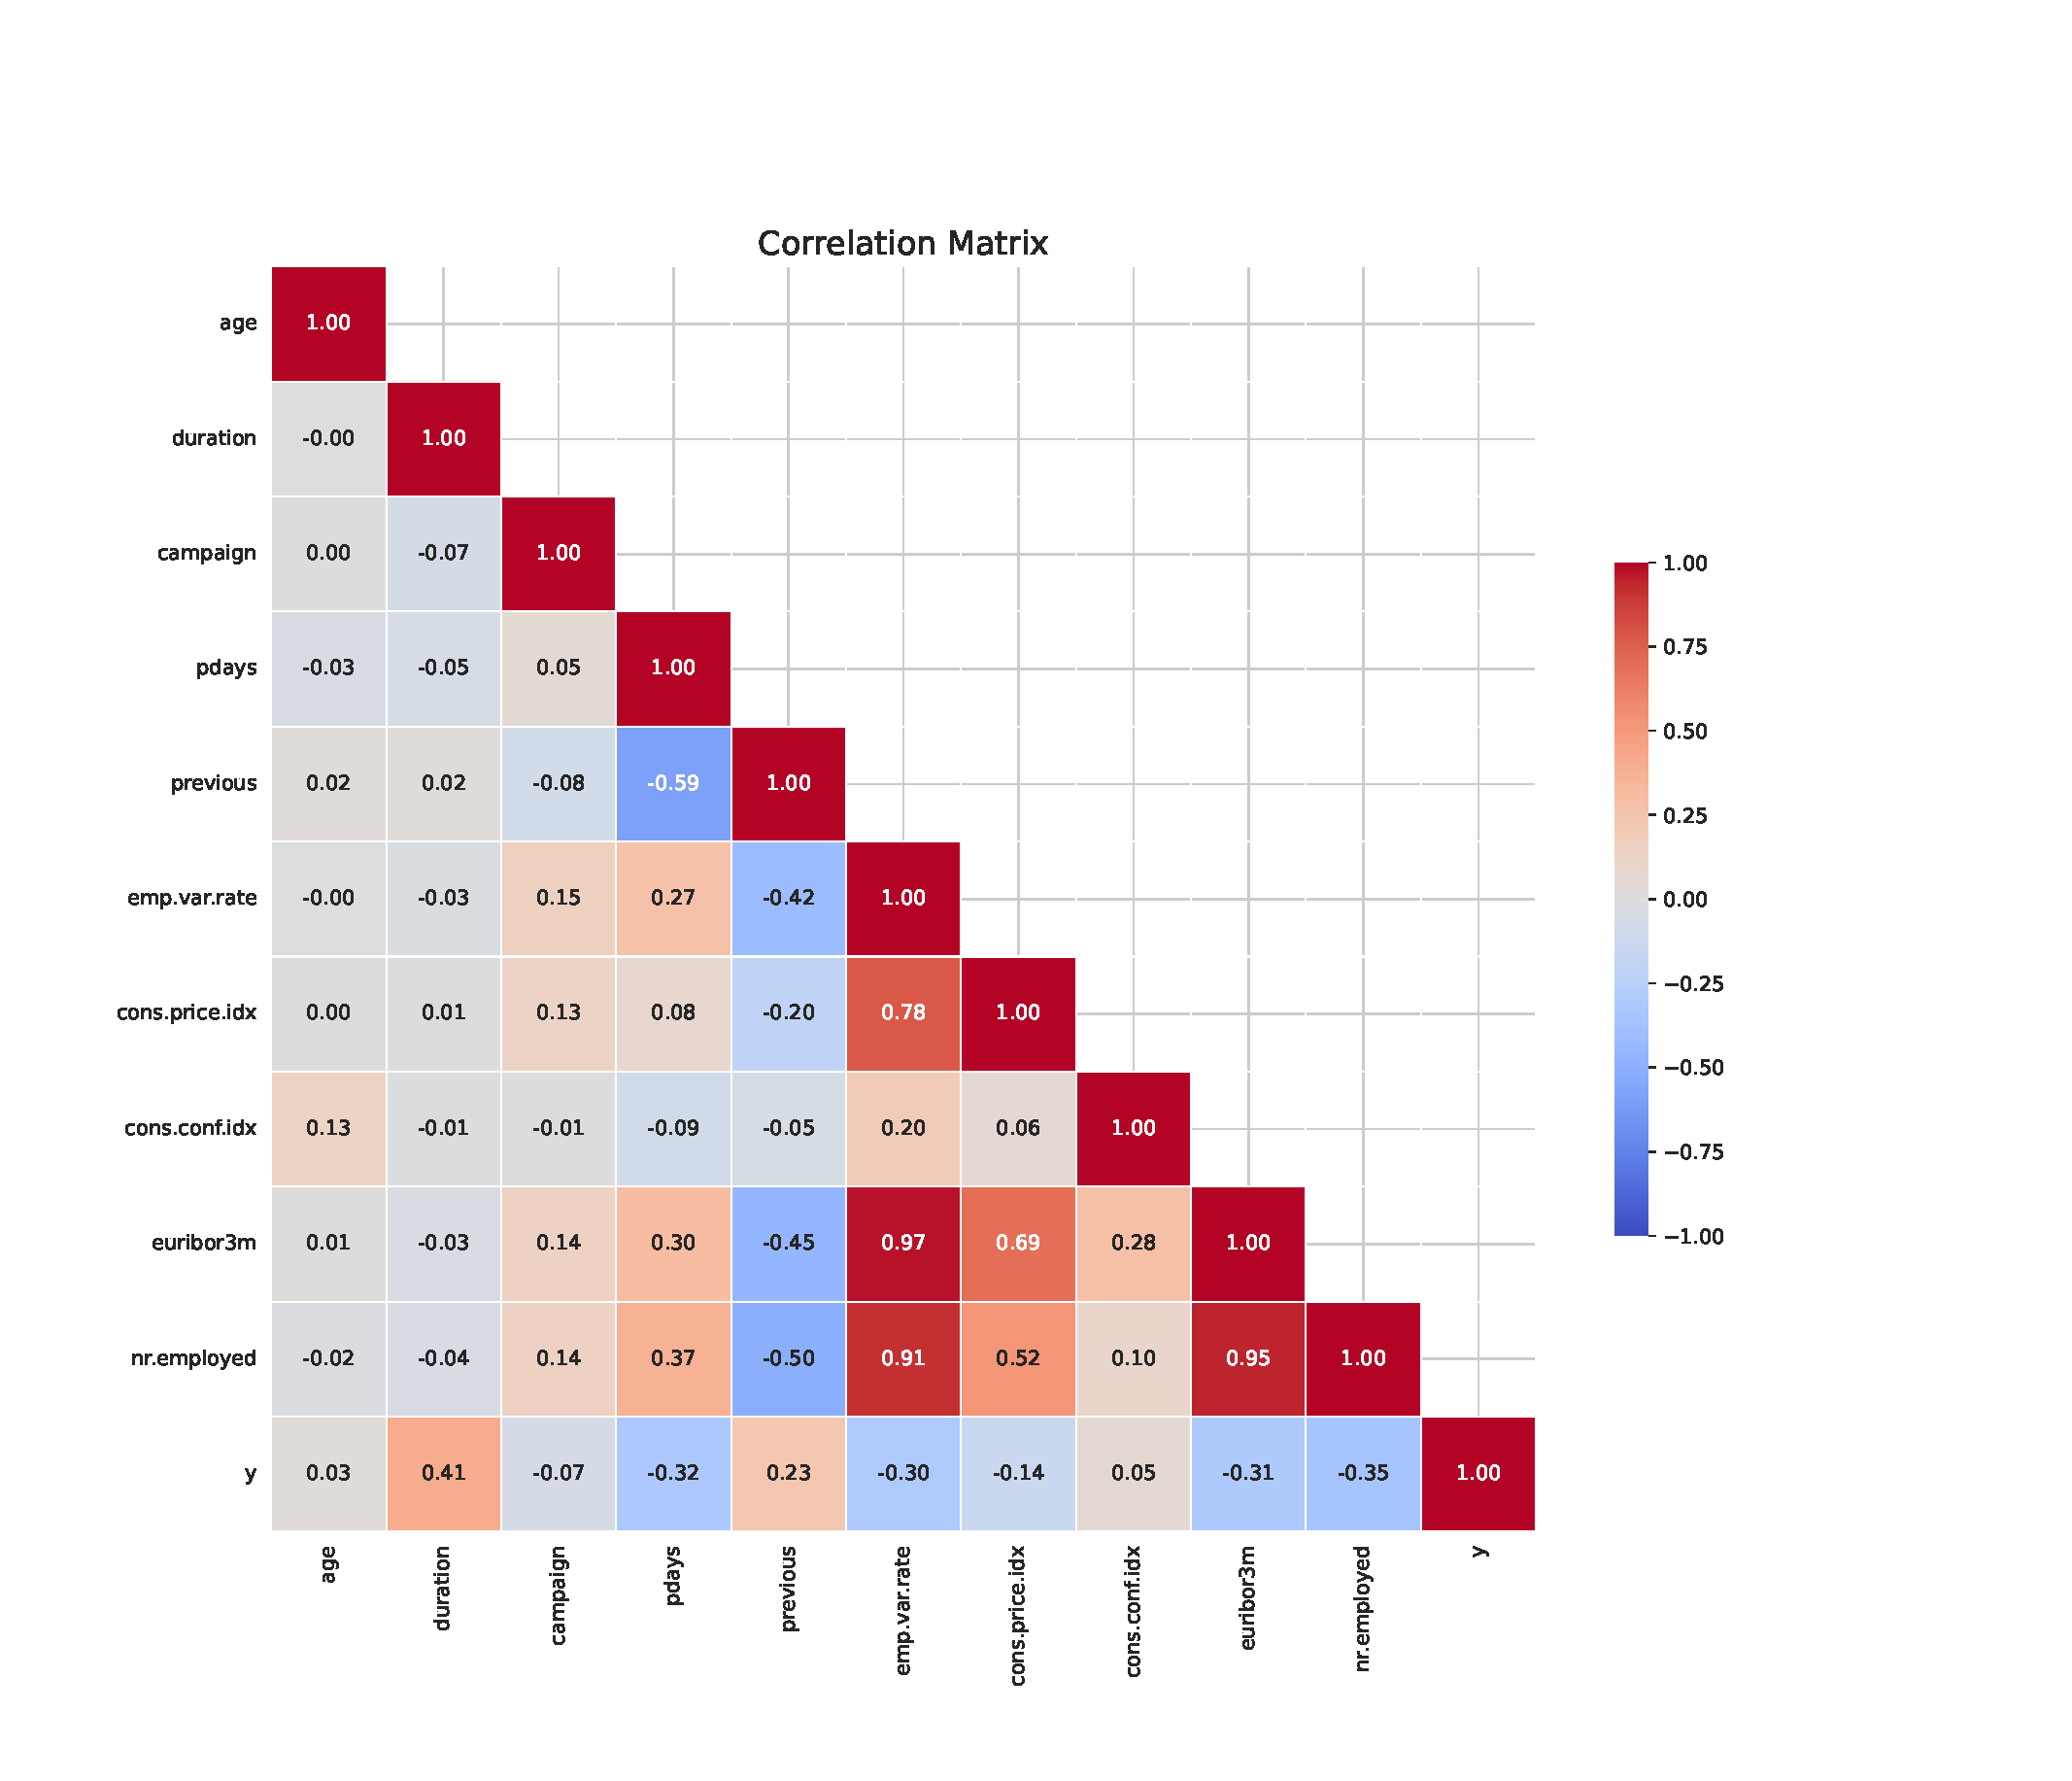
\includegraphics[width=\linewidth]{imagenes/correlation_matrix_lower_triangle_with_diagonal.eps}
		\caption{Correlation matrix of numerical variables. High collinearity justifies the need for dimensionality reduction.}
		\label{figMatrizCorr}
	\end{subfigure}
	
	\begin{subfigure}[b]{0.48\textwidth}
		\centering
		\includegraphics[width=\linewidth]{imagenes/pca_explained_variance.eps}
		\caption{Cumulative explained variance ratio (PCA).}
		\label{figPca}
	\end{subfigure}
	\hfill
	\begin{subfigure}[b]{0.48\textwidth}
		\centering
		\includegraphics[width=\linewidth]{imagenes/claustering.eps}
		\caption{Distribution of the resulting clusters after applying PCA.}
		\label{figClauster}
	\end{subfigure}
	
	\caption{Dimensionality reduction analysis.}
	\label{figAnalisisCompleto}
\end{figure}


\textbf{Comparison: Random Forest, Neural Network, and Stacking:} 

The three models were evaluated using the test set, which preserves the original class imbalance to simulate a real-world scenario. Figure \ref{figROC} shows the comparative ROC curves. It can be seen that the \textbf{Neural Network} model achieved the highest performance with an AUC of 0.9406, slightly outperforming the \textbf{Random Forest} (AUC 0.9359) and the hybrid \textbf{Stacking} architecture (AUC 0.9346). This indicates that the neural network is better at identifying between subscribers and non-subscribers. Figure \ref{figConfusion} shows the comparative confusion matrices between the hybrid architecture (Stacking), which annoyed fewer customers, and the Neural Network, which lost fewer subscribers. When evaluating a high-potential profile (Client A), the architectures differ significantly in their probability estimates. See Table \ref{tab:simulation}\\
% --- Figura 1: Curva ROC ---
\begin{figure}[H]
	\centering
	
	% --- Subfigura 1 (arriba) ---
	\begin{subfigure}[b]{1\textwidth}
		\centering
		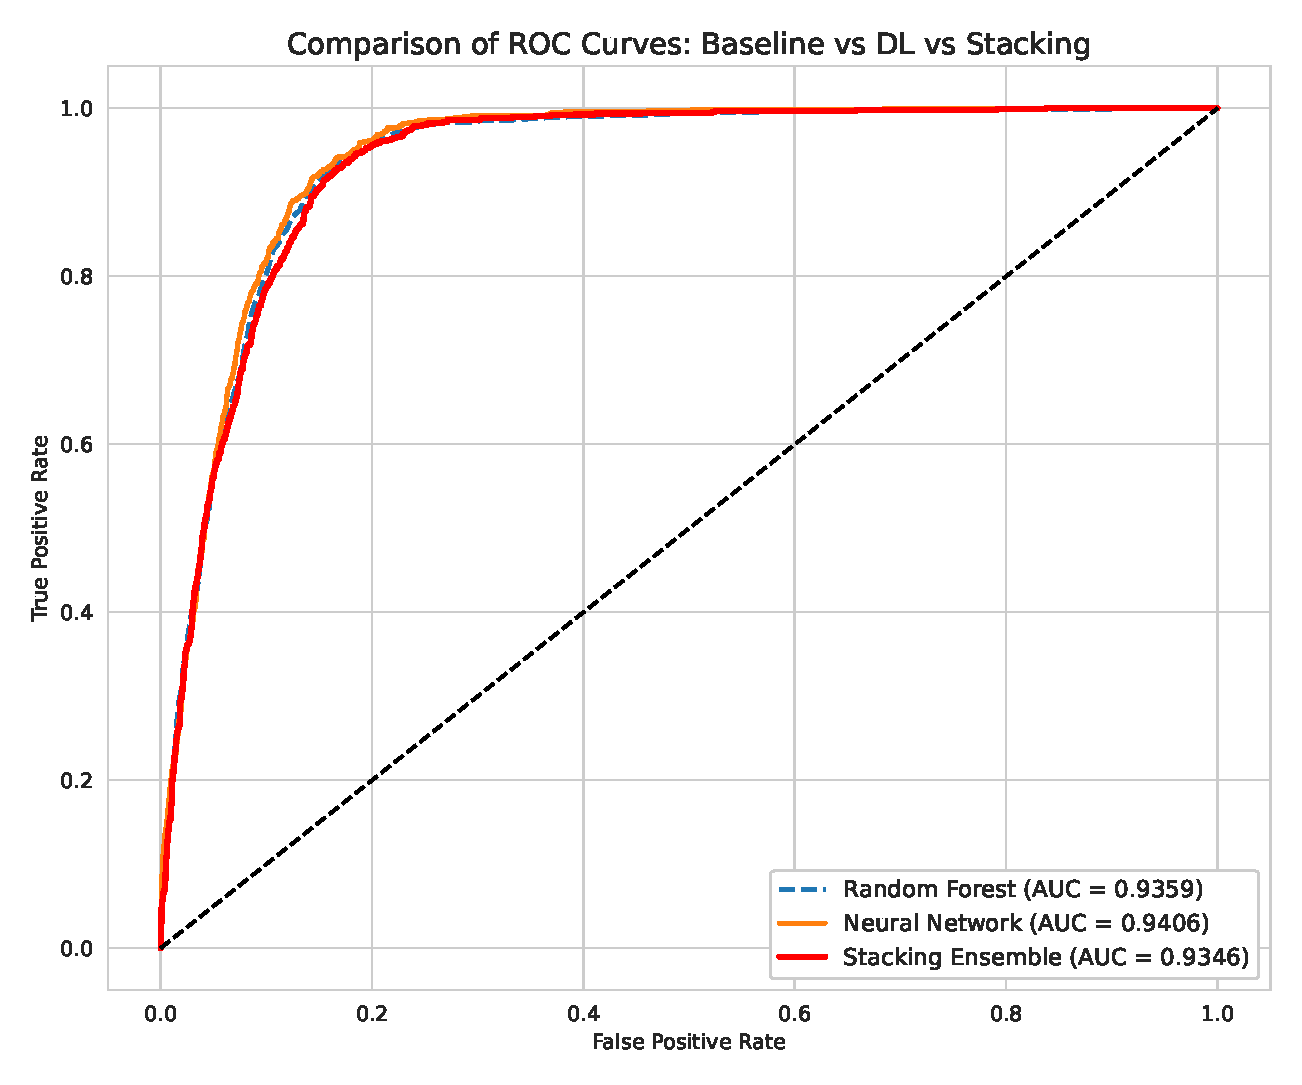
\includegraphics[width=\linewidth]{imagenes/roc_curves.eps}
		\caption{Comparative ROC curves between Baseline and Proposal.}
		\label{figROC}
	\end{subfigure}
	
	\vspace{0.3cm} % espacio vertical controlado
	
	% --- Subfigura 2 (abajo) ---
	\begin{subfigure}[b]{1\textwidth}
		\centering
		\includegraphics[width=\linewidth]{imagenes/matrices_confusion.eps}
		\caption{Confusion matrix of the Neural Network model.}
		\label{figConfusion}
	\end{subfigure}
	
	\caption{Performance evaluation of the proposed model.}
	\label{figPerformance}
\end{figure}

\begin{table}[H]
	\centering
	\caption{Prediction simulation for new customer profiles (Deployment)}
	\label{tab:simulation}
	\begin{tabular}{|l|c|c|c|c|}
		\hline
		\textbf{Customer Profile} & \textbf{Random Forest} & \textbf{Neural Network} & \textbf{Stacking} & \textbf{Consensus} \\ \hline
		
		\begin{tabular}[c]{@{}l@{}}\textbf{Customer A (Potential)}\\ 25 years old, Student, Call: 600s\end{tabular} & 
		\begin{tabular}[c]{@{}c@{}} 57\% \\ \textbf{ACCEPTS} \end{tabular} & 
		\begin{tabular}[c]{@{}c@{}} \textbf{85.4\%} \\ \textbf{ACCEPTS} \end{tabular} & 
		\begin{tabular}[c]{@{}c@{}} 14.3\% \\ \textit{REJECTS} \end{tabular} & 
		{\textbf{No}} \\ \hline
		
		\begin{tabular}[c]{@{}l@{}}\textbf{Customer B (Not interested)}\\ 55 years old, Retired, Call: 100s\end{tabular} & 
		\begin{tabular}[c]{@{}c@{}} 8\% \\ REFUSES \end{tabular} & 
		\begin{tabular}[c]{@{}c@{}} 0\% \\ REJECT \end{tabular} & 
		\begin{tabular}[c]{@{}c@{}} 0\% \\ REJECT \end{tabular} & 
		{Yes}\\ \hline
		
		\textbf{F1-Score} & \textbf{0.6137} & \textbf{0.6285} & \textbf{0.5799} & -- \\ \hline
		
	\end{tabular}
\end{table}


\begin{figure}[H]
	\centering  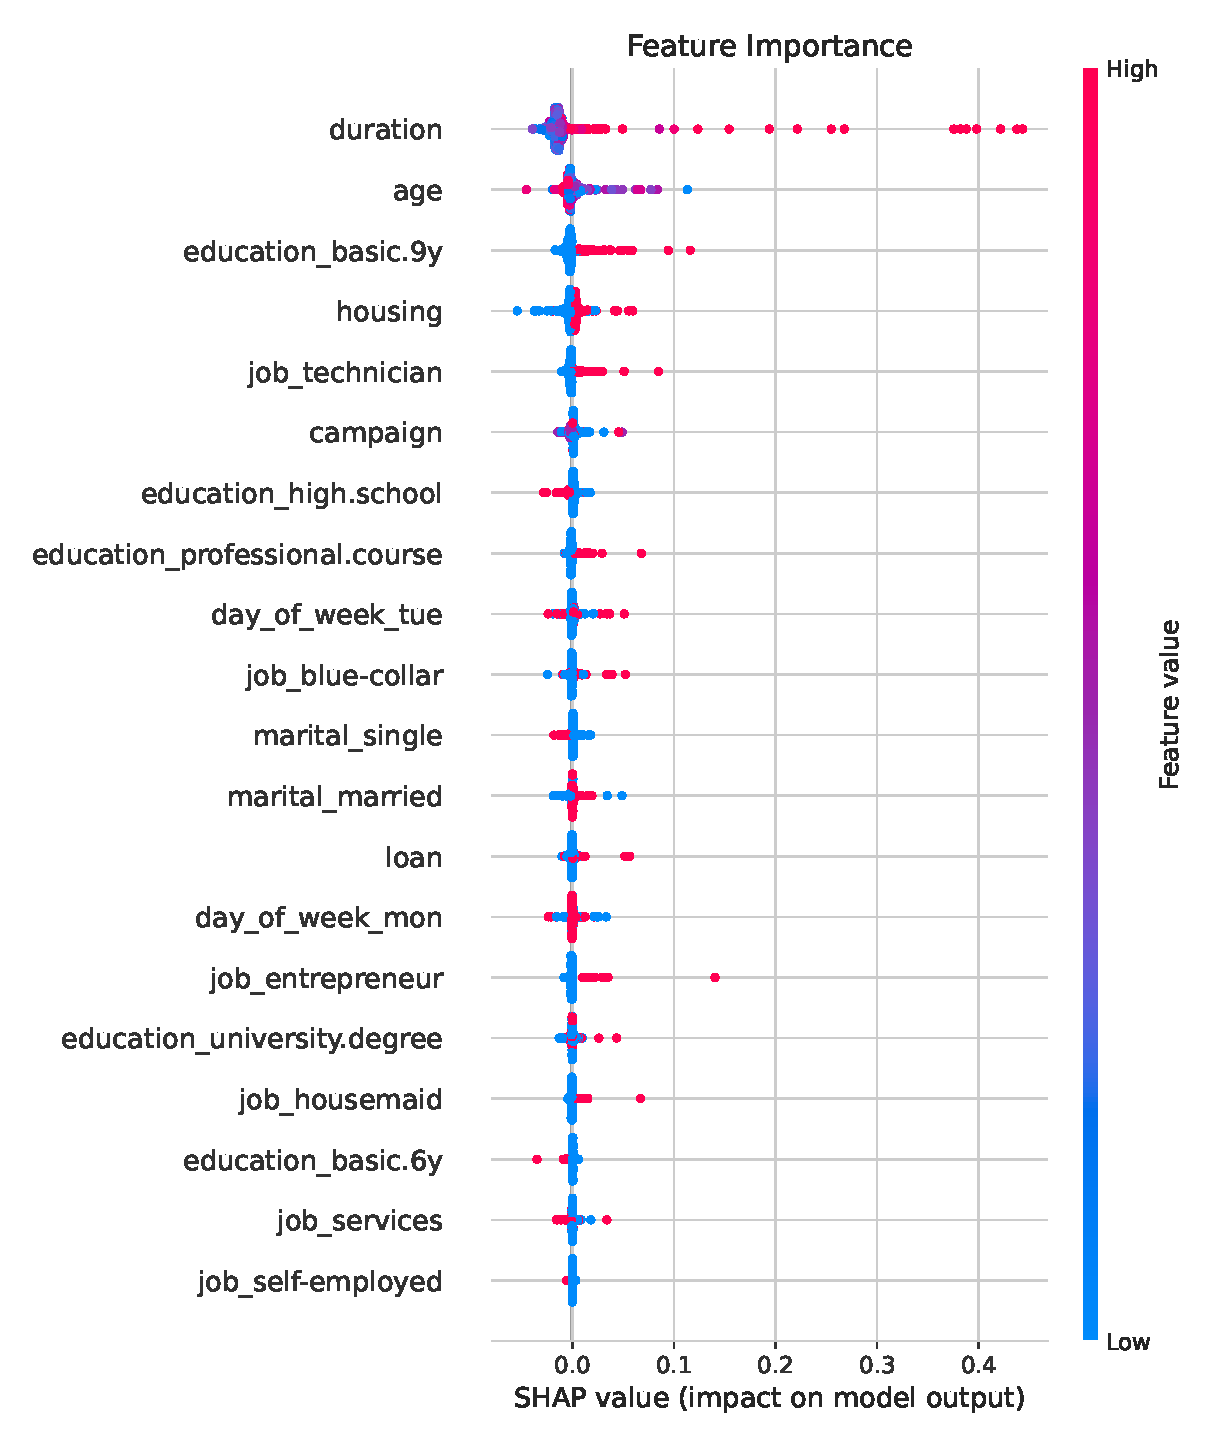
\includegraphics[width=0.8\textwidth]{imagenes/shap_explicability_real_names.eps}
	\caption{Análisis de importancia de características mediante valores SHAP.}
	\label{figSAHP}
\end{figure}


\textbf{Explainability Analysis (XAI):}

For the explainability analysis, a proxy model based on the original data was used. Figure \ref{figSAHP} illustrates the most influential characteristics in the prediction. The analysis reveals that the call duration variable is the strongest predictor: longer calls dramatically increase the probability of success. There are other variables such as age, educational level, and certain job categories that help predict which customers are most likely to accept.

\section{Conclusions}

This study has successfully addressed the challenge of optimizing the prediction of fixed-term deposit subscriptions in the banking sector. The results obtained validate the hypothesis that the incorporation of advanced preprocessing techniques and neural network architectures can outperform traditional approaches and complex ensemble strategies in unbalanced data contexts.\\

In phase 1, the application of PCA allowed the feature space to be compressed from 47 to 22 dimensions and, combined with class balancing using SMOTE, the inherent bias towards the majority class was mitigated, establishing a solid basis for model learning. In phase 2, the Neural Network (ANN) achieved the best overall performance with an AUC-ROC of 0.942, outperforming Random Forest and Stacking. Analysis of the confusion matrix showed that the Neural Network model proved to be operationally superior by minimizing false negatives. This implies a significantly greater ability to capture potential customers, maximizing the campaign's return on investment despite having a slightly higher false positive rate. In phase 3, the incorporation of Explainable Artificial Intelligence using SHAP values was fundamental in demystifying the “black box.” The analysis identified the original variables ($duration$, $age$, $education$) and confirmed that contact duration is the strongest predictor, validating the economic consistency of the model. Finally, the deployment simulation with new customer profiles revealed the limitations of the Stacking model, which tended to be overly conservative in rejecting potential customers, while the neural network demonstrated the flexibility necessary to correctly identify sales opportunities.\\

For future research, it is suggested to explore sequential Deep Learning architectures, such as Recurrent Neural Networks (RNN), to capture the temporality in the history of customer contacts.



%
% ---- Bibliography ----
%
% BibTeX users should specify bibliography style 'splncs04'.
% References will then be sorted and formatted in the correct style.
%
% \bibliographystyle{splncs04}
% \bibliography{mybibliography}
%
\bibliographystyle{splncs04}
\bibliography{references} 

\end{document}

